\documentclass[11pt,a4paper]{article}
\usepackage[margin=1in]{geometry}
\usepackage{graphicx}
\usepackage{amsmath}
\usepackage{array}
\usepackage{booktabs}
\usepackage{tikz}

\parindent=0pt

\newcommand{\emptybox}{%
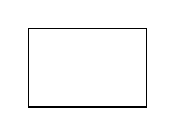
\begin{tikzpicture}[scale=1, baseline=0.2cm]
\draw (0,0)rectangle(1.5,1);
\end{tikzpicture}
}

\title{Keeping Secrets: Cybersecurity and Cryptography\\
\large Cryptography: Public-Key Encryption Activity}
\author{}
\date{}

\begin{document}

\maketitle

\section*{Activity 1: Generating Keys Using Small Integers}

In Activity 1 we use modular product tables to generate our modular inverses.

\begin{enumerate}
    \item First complete the following modular five (M-5) multiplication table:
    
    \begin{center}
    \renewcommand{\arraystretch}{1.5}
    \begin{tabular}{|c|c|c|c|c|c|}
    \hline
    \textbf{M5} & \textbf{0} & \textbf{1} & \textbf{2} & \textbf{3} & \textbf{4} \\
    \hline
    \textbf{0} & \hspace{.6cm} &\hspace{.6cm} &\hspace{.6cm} &\hspace{.6cm} &\hspace{.6cm} \\
    \hline
    \textbf{1} & & & & & \\
    \hline
    \textbf{2} & & & & & \\
    \hline
    \textbf{3} & & & & & \\
    \hline
    \textbf{4} & & & & & \\
    \hline
    \end{tabular}
    \end{center}
    
    \vspace{1cm}
    
    \item Now complete this modular nine (M-9) multiplication table:
    
    \begin{center}
        \renewcommand{\arraystretch}{1.5}
    \begin{tabular}{|c|c|c|c|c|c|c|c|c|c|}
    \hline
    \textbf{M9} & \textbf{0} & \textbf{1} & \textbf{2} & \textbf{3} & \textbf{4} & \textbf{5} & \textbf{6} & \textbf{7} & \textbf{8} \\
    \hline
    \textbf{0} &\hspace{.6cm} &\hspace{.6cm} &\hspace{.6cm} &\hspace{.6cm} &\hspace{.6cm} &\hspace{.6cm} &\hspace{.6cm} &\hspace{.6cm} &\hspace{.6cm} \\
    \hline
    \textbf{1} & & & & & & & & & \\
    \hline
    \textbf{2} & & & & & & & & & \\
    \hline
    \textbf{3} & & & & & & & & & \\
    \hline
    \textbf{4} & & & & & & & & & \\
    \hline
    \textbf{5} & & & & & & & & & \\
    \hline
    \textbf{6} & & & & & & & & & \\
    \hline
    \textbf{7} & & & & & & & & & \\
    \hline
    \textbf{8} & & & & & & & & & \\
    \hline
    \end{tabular}
    \end{center}
\end{enumerate}

\newpage

You will first simulate public key encryption using the second table above: the modular nine multiplication table. Your first `message' must be restricted to an integer between 1 and 8.

\section*{Choose Your Keys}

\begin{enumerate}
    \item Your \textbf{Public key} is the modular multiplication table used. Here it is 9. \hfill 
    
    \item Pick two integers from the table whose mod product is 1 (e.g., 4 and 7).
    
    \begin{enumerate}
        \item Your \textbf{encryption key} is the first integer. \hfill \textbf{Encryption key} \emptybox 
        
        \item Your \textbf{decryption key}, or \textbf{private key} is the second integer. \\
        \phantom{>}\hfill \textbf{Decryption key} \emptybox
    \end{enumerate}
    
    \textbf{You can tell others your public and encryption keys but your decryption key is kept private!}
\end{enumerate}

\section*{Sending and Decoding the Secret Message}

\begin{enumerate}
    \item \textbf{How to encrypt:}
    
    \begin{enumerate}
        \item Choose a `message' for secret transmission (here it needs to be restricted to an integer between 1 and 8). This is the \textbf{message} which we will represent as an integer.
        
        \hfill \textbf{Message} (in the form of an integer) \emptybox
        
        \item Using the modular multiplication table find M-product of the message integer and their encryption key. This result is the \textbf{encoded secret message}.
        
        \hfill \textbf{Encryption key} \emptybox
    \end{enumerate}
    
    \vspace{0.5cm}
    
    \item \textbf{How to decrypt:}
    
    Use the M9 table to find the M-product of the decryption (private) key and the encrypted message. This is the decrypted message, known only to those who have the private key.
    
    \hfill \textbf{The decrypted message} \emptybox
\end{enumerate}

\vspace{1cm}

Real-life encryption with public and private keys also uses modular arithmetic. However, we know the table and we know there are very few choices for the multiplicative modular inverses.

It would not be hard for someone to guess our message. In real life, encryption uses far larger numbers that would be very hard to guess.

In the next Activity we will use much larger numbers.

\vfill

\noindent\small
\textcopyright{} 2016 Education Services Australia Ltd, unless otherwise indicated.\\
Creative Commons BY 4.0 license, unless otherwise indicated.

\end{document}
